%!TEX root = ../thesis.tex
%*******************************************************************************
%****************************** Third Chapter **********************************
%*******************************************************************************

\chapter{A more direct approach}
\label{chap:direct_approach}

\ifpdf
    \graphicspath{{Chapter3/Figs/Raster/}{Chapter3/Figs/PDF/}{Chapter3/Figs/}}
\else
    \graphicspath{{Chapter3/Figs/Vector/}{Chapter3/Figs/}}
\fi


\topic{A simple but efficient solution is to map the input data to the target with a neural network whose architecture and training procedure are carefully chosen.}

\cecile{Pourquoi on choisit les MDN et pourquoi on combine avec l'architecture Neural statistician n'est pas clair.}
\cecile{Changer le nom de "mixture model" car ça fait penser au génératif.}
\cecile{Une grade partie du chapitre de parle pas de variance. Il faut citer la mesure de la variance bcp + tôt !}



\section{Motivation} % (fold)
\label{sec:motivation}

\topic{Although the generator is available classical Bayesian inference is difficult because of the intractable likelihood.}







\subsection{Likelihood free} % (fold)
\label{sub:likelihood_free}


A generative model $G(\mu)$ is available to simulate the studied process and retrieve the observations $x$ from given parameters $\mu$.
The objective is to reverse the generator $G^{-1}(x)$ to access the quantities of interest ruling the process.

Since the process is stochastic the generator can produce different observations from the same parameters.
The probability of observing $x$ if the generator is fed with $\mu$ is $p(x | \mu)$.
Therefore reversing the generator means finding $p(\mu | x)$.
From Bayes theorem we get :

\begin{equation}
    p(\mu | x) = \frac{p(x | \mu) p(\mu) }{p(x)}
\end{equation}
Unfortunately the likelihood $p(x | \mu)$ is often intractable because of high dimensional integrals (see \autoref{sub:inverse_problem} and \autoref{sub:simulation}).
Instead of replacing the likelihood or trying to regress it we propose to directly approximate the posterior $p(\mu | x)$ with a sufficiently powerfull and tractable distribution $q_\phi(\mu | x)$.

\autoref{chap:intro_stat} showed a workaround for the study of a mixture coefficient of a Poisson counting process.
This chapter presents an inference method which does not require more domain knowledge than the simulator itself and may be applied on any parameter of interest, not only a mixture coefficient.







\subsection{Core idea} % (fold)
\label{sub:core_idea}

The parameter of interest impact is not on the observables $x$ but on the distribution of the observables $p(x|\mu)$.
This is invisible at the sample scale.
With only one sample $x$ it is not possible to get knowledge on the parameter $\mu$.
Measuring properties of the distribution is only moving the problem from a sample scale to a dataset scale.

The learning problem is to get from an empirical distribution $D = \{x_i\}_{i=0}^N \in \RR^{d\times N}$ to a real number $\mu \in \RR$.
This is a regression problem.
The training algorithm and architecture details is left in \autoref{sec:regression}.
A training or testing dataset is then a set of pairs $\{(D_i, \mu_i)\}_{i=0}^M$.

To avoid confusion between the dataset $D_i$, which is now a data point, and the dataset $Train = \{(D_i, \mu_i)\}_{i=0}^M$ we will call in this chapter $D_i$ a sampleset and $Train$ a dataset.

The training and testing datasets can be obtained by sampling the parameter from a prior distribution then using the simulator to transform this parameter to its corresponding dataset.

The last detail to take care of is the size of the sampleset.
The ideal size is the expected size of the experimental data or a range of possible data size.
But it may be too large to train a neural network with available computation power in a reasonable time.
The size of the sampleset is then a tradeoff between the size of the experimental dataset and available computation power.

\begin{algorithm}[H]
 M $\gets$ dataset size \;
 Dataset $\gets []$ \;
 \For{$i \in [0, M]$}{
 $N \gets$ sample size \;
  $\mu_i$    $\gets$ sample from $p(\mu)$ \;
  $D_i \gets []$ \;

 \For{$j \in [0, N]$}{
  $x_j$  $\gets$ sample from $G(\mu_i)$ \;
  $D_i$.append( $x_i$ ) \;
  }
 Dataset.append ( $(D_i, \mu_i)$ ) \;
 }
 \caption{Generating dataset}
\end{algorithm}








\subsection{Simple workflow} % (fold)
\label{sub:simple_workflow}

The workflow presented in \autoref{chap:intro_stat} relies on several steps : simulator, classifier, likelihood and optimizer.
The final inference suffers from the accumulation of sub-optimality of these steps.
Which is why each step receives special care.
This can be quite expensive and sometimes reaching a near optimal process is not possible.

The proposed workflow is simpler and relies only on a simulator and the training of a regressor.
Mathematical modeling will always be more accurate than an approximate model obtained with machine learning.
Making mathematical modeling the first method to try anyway.
When mathematical modeling is flawed with too expensive computation power or irrealistic approximations then machine learning may be a better approach.

This new workflow moves the computation power of the optimization process from inference (maximum likelihood optimization) to training (back-propagation) leading to faster inference once put in production.

Analysis of the final data obtained at the LHC can leverage long computation on a cluster.
But the speed of inference is critical for the high level trigger of the LHC where decisions must be made.
Other domains as high frequency trading, web advertising recommandation, real time applications also requires fast inference.




\section{Regression} % (fold)
\label{sec:regression}




\topic{Mixture density networks are a tractable but powerful tool to approximate a conditional probability density.}



\subsection{Density networks} % (fold)
\label{sub:density_networks}

% subsection density_networks (end)
\topic{Approximate the posterior with a very powerfull and flexible model}

A way of approximating the posterior $p(\mu | x)$ is to define a tractable but flexible enough family of distribution $q_\phi(\mu | x)$ parametrized by $\phi$.

Initially introduced in \cite{Bishop94mixturedensity} as a generalization of least square methods to train neural network, mixture density networks (MDN) can be made as powerful as required while staying tractable.
Used as a regressor MDN allows to estimate both the expected value and its uncertainty as detailed is \autoref{sub:extract_parameters}.

The target density is approximated by a linear combination of kernels $k$ :

\begin{equation}
    q_\phi(\mu | x) = \sum_{i=0}^K m_i(x ; \phi) k_i(\mu | x ; \phi)
\end{equation}
where $m_i(x ; \phi)$ are the mixture coefficient
and the kernels $k_i(\mu | x ; \phi)$ usually chosen as Gaussian :
\begin{equation}
    k_i(\mu | x ; \phi) = \frac{1}{\sigma_i(x ; \phi) \sqrt{2 \pi}} e^{- \frac{1}{2} \left ( \frac{\mu-y_i(x ; \phi)}{\sigma_i(x ; \phi)} \right )^2} 
\end{equation}

$m_i(x ; \phi)$, $\sigma_i(x ; \phi)$ and $y_i(x ; \phi)$ are the outputs of a neural network, whose parameters are gathered in $\phi$, and taking the data as input.
Finally, the mixture coefficient have to sum up to 1.
\begin{equation}
    \sum_{i=0}^K m_i(x ; \phi) =  1
\end{equation}

The motivation for this approximation is twofold.
First, given enough well chosen parameters a Gaussian mixture model can approximate any density.
Second, a neural network with enough hidden unit is able to approximate any continuous function with arbitrarily precision.
Combining these two properties leads to an arbitrarily powerful approximation of any conditional density $p(\mu|x)$ given enough resources.








\subsection{Training principle} % (fold)
\label{sub:training_principle}

\topic{MDN are trained like classical regressor and allow to compute the uncertainty of the predictions.}
The neural network parameters $\phi$ can then be obtained by maximizing the likelihood that the model produced the given data.

\begin{equation}
    \phi^\star = \argmax_\phi \mathcal L (\phi)
\end{equation}
\begin{equation}
    \mathcal L (\phi) = \sum_{i=0}^K m_i(x ; \phi) k_i(\mu | x ; \phi)
\end{equation}


For convenience the optimization is usually turned into a minimization of the negative log likelihood (NLL) :
\begin{equation}
    \phi^\star = \argmin_\phi - \log \mathcal L (\phi)
\end{equation}

In the simple case of one Gaussian component ($K=1$) the NLL is :
\begin{equation}
    \phi^\star = \argmin_\phi \left\{ \log(\sigma(x;\phi)) + \frac{1}{2}\log(2\pi) + \frac{(\mu^\star - y(x;\phi))^2}{2\sigma(x;\phi)^2} \right\}
\end{equation}

Similarly to training a regular neural network regressor with least square, MDN's training is supervised.
Therefore requires data for which the ground truth is available which is verified in our case since we need both observed data $x$ and the associated value for  $\mu^\star$.

Finally the likelihood, with Gaussian kernels, is fully differentiable making possible the use of stochastic gradient descent methods to obtain the neural network parameters $\phi$.


\begin{algorithm}[H]
 \For{$i \in [0, N]$}{
  $\mu_i$    $\gets$ sample from $p(\mu)$ \;
  $x_i$      $\gets$ $G(\mu_i)$ \;
  $m_i, y_i, \sigma_i$ $\gets$ $f(x_i; \phi_i)$ \;
  $loss_i$   $\gets$ $-\log \mathcal L(\phi_i; m_i, y_i, \sigma_i)$ \;
  $grads_i$  $\gets$ backward($loss_i$) \;
  $\phi_{i+1}$ $\gets$ Optimizer($\phi_i$, $grads_i$) \;
 }
 \caption{Training procedure}
\end{algorithm}







\subsection{Architecture details} % (fold)
\label{sub:architecture_details}

The requirement that the mixture coefficients $m_i$ sum up to 1 is enforced using softmax operator on the $K$ output neurons representing the $m_i$.
Similarly the standard deviation of Gaussians should always be strictly positive which is fulfilled by interpreting the neuron output as $\log(\sigma_i)$.
No particular operation are necessary on the mean $y_i$ of the Gaussians since it can take whatever real value.


\victor{TODO : Un dessin ?}





\subsection{Training details} % (fold)
\label{sub:training_details}

One particularity of the MDN with gaussian kernels is the difference between the convergence speed of the mean and the variance 

\begin{equation}
    loss = \textcolor{myred}{\log(\sigma(x;\phi))} + \frac{\textcolor{myblue}{(\mu^\star - y(x;\phi))^2}}{2\textcolor{mypurple}{\sigma(x;\phi)}^2}
\end{equation}

At the begining of training the predicted mean $y$ is far from the truth $\mu^\star$.
The \textcolor{mypurple}{purple} term tries to compensate for the \textcolor{myblue}{blue} term leading to a fast increase of $\sigma$ to while the regressor moves to better predictions.
The constrain of the \textcolor{myred}{red} term is negligeable because of its log scale.

Once better predictions occur more often the constrain on $\sigma$ ($\textcolor{myred}{\log(\sigma(x;\phi))}$) slowly (still log scale) narrow the output probability density near the correct value of $\mu^\star$.

This leads to bouncing loss when Adam optimizer \needcite is used with default parameter because the inertia of the gradient descent is too high.
The gradient descent of the neural network parameter is bouncing back and forth around some local minimum without reaching convergence.

To fix this issue $\beta_1$ and $\beta_2$ must be set to lower values to reduce inertia.
Typically $\beta_1=0.5$ and $\beta_2=0.9$.

\victor{TODO : ajouter un graphique de la loss qui rebondi. et un avec la loss qui rebondi pas}

Even if the inertia of the optimizer is fixed outliers can lead to unstable training.
Many steps without outliers will make the network overconfident ie narrow down the estimated variance of prediction.
Once an outlier appear in some mini-batch the average loss will go up and $\sigma$ may jump to higher values.
Again many steps without outliers reduces $\sigma$ until a new outlier appear, and so on.
If the criterion to stop training leads does not take into account this effect the performances of the MDN is stained with randomness.

Fixing this issue requires to make sure that the mini-batches are representative of the true distribution of the data.
Simply increasing the mini-batch size is often enough.

The 2 issues presented here may occure even for the simple case of one Gaussian kernel.
This may explain why MDN are not so popular in the deep learning community.






\subsection{Extract parameters} % (fold)
\label{sub:extract_parameters}

\topic{We have access to the full posterior (formulas included). So parameter estimation is now easy}


As long as a flexible and powerful enough parametric differentiable function is mapping the data $x$ to the parameter $\mu$ it is possible to approximate the conditional density.
Once trained the inference is straightforward since closed formulas are available.


\subsubsection{Extract moments} % (fold)
\label{ssub:extract_moments}

From the experimental data $x^\star$ the mean and variance can be easily extracted using usual formulas for mixture models \needcite :

\begin{align}
    \bar \mu & = \mathbb E_{p(\mu | x^\star)}[\mu] \\
    & \approx \mathbb E_{q_\phi(\mu | x^\star)}[\mu] \\
    & = \sum_{i=0}^K m_i(x^\star ; \phi) \int d\mu ~ \mu ~ k_i(\mu | x^\star ; \phi) \\
    \label{eq:extract_mean}& = \sum_{i=0}^K m_i(x^\star ; \phi) y_i(x^\star ; \phi)
\end{align}

\begin{align}
    \Delta\mu^2 & = \mathbb V_{p(\mu | x^\star)}[\mu] \\
    & \approx \mathbb V_{q_\phi(\mu | x^\star)}[\mu] \\
    & = \sum_{i=0}^K m_i(x^\star ; \phi) \int d\mu ~ \mu^2 ~ k_i(\mu | x^\star ; \phi) - \bar \mu^2 \\
    \label{eq:extract_sigma} & = \sum_{i=0}^K m_i(x^\star ; \phi) \left [ \sigma_i(x^\star ; \phi)^2 + y_i(x^\star ; \phi)^2 - \bar \mu^2 \right ]
\end{align}

The last step (\autoref{eq:extract_mean} and \autoref{eq:extract_sigma}) assumes that the kernels are all gaussian.

Of course if the target distribution is a simple gaussian the mean and standard deviation are directly computed by the neural network.

\subsubsection{Extract modes} % (fold)
\label{ssub:extract_modes}

As seen in \autoref{sub:classic_parameter_estimation} the mode of posterior distribution may be prefered to the full distribution itself.
There is no formulas to extract modes from a mixture of distribution even if all the sub-distribution are gaussian.
However all the parameters of our mixture distibution are known making fast otimization to search for maxima possible but also sampling from this distribution to estimate its properties.

A simple example : the search of a global maximum can be approximated by the highest value of a histogram built on a very large sample from the mixture distribution.
Sampling from a mixture of a dozen gaussians is way cheaper than running a signle full simulation of the process.
Moreover this naive approximation can be used to narrow down the search using optimization.








\subsection{Datasetwise input} % (fold)
\label{sub:datasetwise_input}

\topic{Neural network using reduction function, such as the average, can extract complex link between the parameters of a generative distribution and a dataset which is a realisation of this distribution.}
\topic{Independent measurement requires permutation invariant functions}

In order to accurately capture the complex mapping between the data and the parameters the architecture of the neural network should embody the constraints of the chosen family distribution.

If the studied process is stochastic the observations are usually composed of repeated independent measurements of an event.
Then the observable is not a real valued vector $\xx \in \RR^d$ but a set of data points $D = \{\xx_i \in \RR^d \}_{i=0}^N$.
The output is still a real valued vector meaning that the neural network architecture should include some reduction function to map the set of vector $D$ to a single vector $\yy$.
Usual candidates are averages, minima, maxima, products, sums, geometric means or others that reduce the dimension and remain invariant to the input order of the input vectors.
In practice the average is the favorite one \needcite.

Section 7 of \cite{lucas:hal-01791126} gives a proof that the given \emph{"permutation invariant neural networks"} architecture is a universal approximator of permutation invariant functions.

The \autoref{fig:average_layer} summaries \textbf{one layer} of such neural network.
\begin{figure}[htb]
    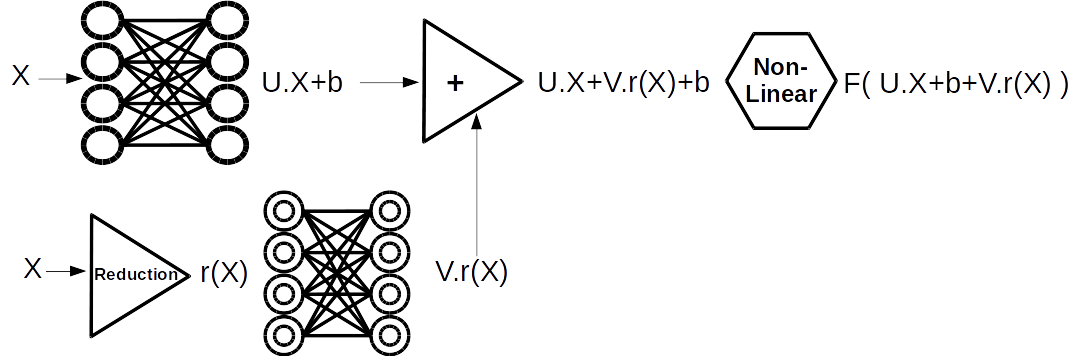
\includegraphics[width=\linewidth]{average_layer}
    \caption{Single layer of the datasetwise neural network. $U$ and $V$ are 2 matrices of the same shape. $r(X)$ is the result of the reduction of the input data $X$. In practice the + operator is relying on broadcasting to sum $V.r(X)$ or $b$ to each sample in $U.X$.}
    \label{fig:average_layer}
\end{figure}



An input sampleset $X$ is analogus to a mini-batch in classical neural network training since it is a matrix of shape $n \times d_0$ with $n$ the number of samples and $d_0$ the number of dimension of a sample.

Reminder : a fully connected single layer neural network is composed of a matrix weight $U \in \RR^{d_0\times d_1}$, a bias vector $b \in \RR^{d_1}$ and a non linearity function $F : \RR^{d_0\times d_1} \to \RR^{d_0\times d_1}$.
The output of a fully connected layer is $ F(U.X+b) \in \RR^{N \times d_1}$.
There is an implicit broadcasing in the sum $(U.X)+b$ since $b$ is a vector and $U.X$ is a matrix.

Here the layer is augmented with another weight matrix $V  \in \RR^{d_0\times d_1}$ and a permutation invariant reduction function $r : \RR^{N \times d_0} \to \RR^{d_0}$.
The output is $ F(U.X+b+V.r(X)) \in \RR^{N \times d_1}$.
The sum $(U.X+b) + (V.r(X))$ involves the same broadcasting as the one between the bias $b$ and $U.X$.








\subsection{Sample weights} % (fold)
\label{sub:sample_weights}

\topic{Weighted instances requires weighted reduction functions}

When the studied process includes some very rare events the simulation uses importance sampling \needcite. 
The simulation output includes importance weights to allow many rare events to be produced while keeping the distribution of events similar to reality.
The neural network must take into account the importance weights to accurately regress the parameters.
Which leads to use weighted average instead of simple average for example and makes maximum and other unweighted reduction ill-suited to this setting.

More precisely, for 2 samplesets $D$ and $D^\prime$ if the associated empirical distribution are equal then the neural network output should also be equal.

\begin{equation}
    \forall x, p_D(x) = p_{D^\prime}(x) \implies f(D; \phi) = f(D^\prime; \phi)
\end{equation}

with,
\begin{equation}
    p_D(x) = \sum_{v \in D} w_i \delta (x - v)
\end{equation}
and $\delta$ is the Dirac distribution function.

\begin{figure}[htb]
    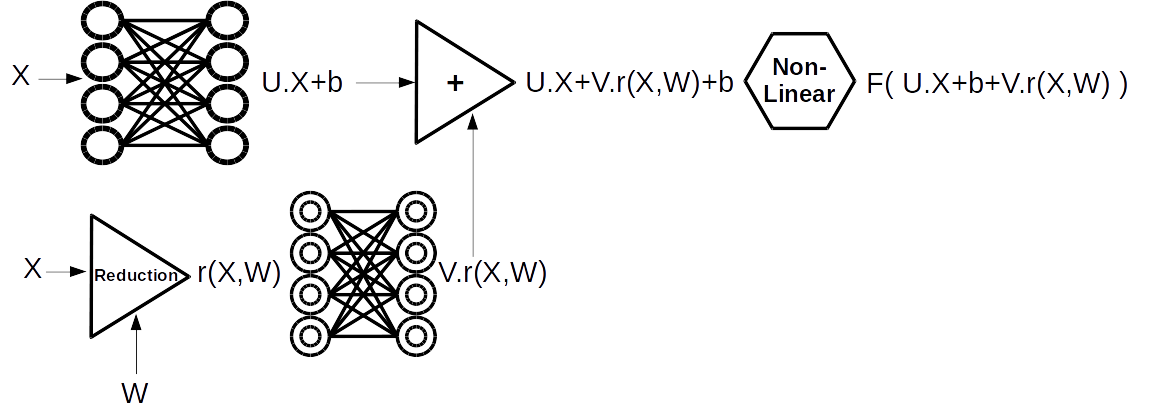
\includegraphics[width=\linewidth]{weighted_average_layer}
    \caption{Single layer of the weighted datasetwise neural network. The reduction function takes into account the sample weights.}
    \label{fig:weighted_average_layer}
\end{figure}







\subsection{Handle nuisance parameter} % (fold)
\label{sub:handle_nuisance_parameter}

The objective is to infer the parameter $\mu$ of a model that describes a stochastic system from experimental data $D^\star$.
However $\mu$ alone is not enough to describe the experimental data.
More causal parameters, noted $\alpha$, are required.
Since the parameters $\alpha$ are not the object of study they are tagged as \emph{nuisance} parameters in opposition to the parameter \emph{of interest} $\mu$.

Until now nuisance parameters were ignored for simplicity.
This section describes two ways to handle nuisance parameters when learning direct regression of the parameter of interest.





\subsubsection{Ignore them} % (fold)
\label{subsub:ignore_them}

\topic{The model can simply learn the marginal posteriors "like a boss"}

The first way is to simply ignore them and directly approximate the marginal posterior $p(\mu|D)$.
The training dataset should include a representative set of samplesets for the problem.
Meaning that instead of simply sampling a new value $\mu_i$ for each sampleset $D_i$ also sample the nuisance parameters from theirs prior distribution to feed them to the simulator $D_i = G(\mu_i, \alpha_i)$.

\begin{algorithm}[H]
 M $\gets$ dataset size \;
 Dataset $\gets []$ \;
 \For{$i \in [0, M]$}{
 $N \gets$ sample size \;
  $\mu_i$    $\gets$ sample from $p(\mu)$ \;
  $\alpha_i$    $\gets$ sample from $p(\alpha)$  \# new \;
  $D_i \gets []$ \;

 \For{$j \in [0, N]$}{
  $x_j$  $\gets$ sample from $G(\mu_i, \alpha_i)$  \# new \;
  $D_i$.append( $x_i$ ) \;
  }
 Dataset.append ( $(D_i, \mu_i)$ ) \;
 }
 \caption{Generating dataset}
\end{algorithm}


The regressor is supposed to internaly handle the impact of the nuisance parameters.
This puts all the pressure of systematic effect on the training which may be too much to allow accurate learning.






\subsubsection{Marginalization} % (fold)
\label{subsub:marginalization}

\topic{Nuisance parameters are marginalized using Monte Carlo integral approximation.}

The other way is to learn the posterior $p(\mu | D, \alpha)$ then to marginlaize the nuisance parameters.
\begin{equation}
    p(\mu | D) = \int d\alpha ~ p(\alpha | D) ~ p(\mu | D, \alpha)
\end{equation}

This integral can be approximated with Monte Carlo.

\begin{equation}
  \int \int d\alpha ~ p(\alpha | D) ~ p(\mu | D, \alpha)
  \approx \sum_i w_i ~ p(\mu | D, \alpha_i)
\end{equation}

Where $p(\mu | D, \alpha)$ is approximated using a trained MDN as seen in the previous sections.
In the case of a MDN $f$ with gaussian kernels, $f$ produces the mixture parameters $m_i, y_i, \sigma_i$ from the experimental data $D^\star$ and sampled $\alpha$.

\begin{algorithm}[H]
 \For{$i \in [0, N]$}{
  $\alpha_i, w_i$ $\gets$ MC sample from $p(\alpha)$ \;
  $\{m_j, y_j, \sigma_j\}_{j=0}^K = f(D^\star, \alpha; \phi^\star)$ \;
  $\bar\mu = \sum_{j=0}^K m_j y_j $ \;
  $\Delta\mu = \sum_{j=0}^K m_j \left [ \sigma_j^2 + y_j^2 - \bar \mu^2 \right ]$ \;
  $\hat\mu$  $\gets$ $\hat\mu + w_i \times \bar\mu$ \;
  $\hat\sigma$  $\gets$ $\hat\sigma + w_i \times (\bar\mu^2 + \Delta\mu^2)$ \;
 }
$\hat\sigma$  $\gets$ $\hat\sigma - \hat\mu^2$ \;
\caption{Marginalizing the nuisance parameters $\alpha$ using MC to compute the integral.}
\end{algorithm}







\section{Discussing the related work} % (fold)
\label{sec:discussing_the_related_work}

\subsection{Similar architecture} % (fold)
\label{sub:similar_architecture}

Causal parameters are often related to properties of the distribution of the data in statistical simulations.
The architecture should reflect this link in order for a neural network to capture the relevant information.
This work is using Mixture density network \cite{Bishop94mixturedensity} combined with neural network architectures design to learn summary statistics on datasets.

Neural Statistician \cite{Edwards17neuralstatistician} is also relying on a similar neural network architecture in the context of transfer learning and one shot learning, where the neural network is producing summary statistics to embed the link between similar datasets.
The idea in Neural Statistician is that similar datasets can be gathered as originating from the same generative model including a global parameter to control the shift between domains.

In this work the architecture is slightly improved to take into account importance weights.
Moreover the objective is completely different since we consider supervised regression.


Another paper \cite{lucas:hal-01791126} is using this architecture to do regression as an adversarial network to reduce mode dropping in generative network.
The adversarial network is encouraged to capture the difference between the real and the fake image distribution by predicting the ratio of fake images in a mini-batch.
This is an inference of a mixture coefficient on an empirical distribution which is exactly the objective given in this work, only missing the estimation of a confidence interval for the predicted mixture coefficient.

Learning to Pivot \cite{louppe_learning_2016} uses a MDN with a mixture of gaussians as adversarial networks in one example.
Pivot adversarial network could also profit from the dataset wise architecture.


\victor{ TODO : And bio-informatic : ask Théo.}


\subsection{INFERNO} % (fold)
\label{sub:inferno}

Using a neural network to directly map the dataset to the estimated parameter distribution can be viewed as an extension of the work done in INFERNO \cite{DECASTRO2019170inferno}. 
INFERNO leverage the domain knowledge of the likelihood at a dataset level to compute a lower bound of the total variance of the maximum likelihood estimator (see \autoref{sub:inferno}).
Allowing the neural network to produce histogram like summary statistics while reducing the uncertainty on the parameters of interest estimation.

The method presented in this chapter can be seen as an extension of INFERNO without the domain knowledge of the likelihood.

In addition INFERNO is producing a function $ F : D \in \RR^{N\times d} \to v \in \RR^k $ which is exactly what the samplesetwise architecture is doing.
Meaning that the neural network layer architecture described in \autoref{sub:datasetwise_input} can be used with INFERNO to produce arbitrary complex permutation invariant histogram-like functions.

Although the regressor is trained using some chosen likelihood it is not straightforward that the inferno loss can be applied here too.


\subsection{Neural network uncertainty} % (fold)
\label{sub:neural_network_uncertainty}

The choice of mixture density network to measure the uncertainty is completly arbitrary.
Other methods to compute neural network prediction uncertainty are available and should be cited as well.


\victor{TODO : beaucoup trop d'articles à lire sur le sujet.}
From \url{https://arxiv.org/pdf/1906.02530.pdf} :
\begin{itemize}
	\item MDN (MacKay \& Gibbs, 1999)
	\item aleatoric uncertainty(Kendall \& Gal, 2017)
	\item Bayesian approache : Laplace approximation (MacKay, 1992)
	\item variational inference (Graves, 2011; Blundell et al., 2015)
	\item dropout-based variational inference (Gal\& Ghahramani, 2016; Kingma et al., 2015)
	\item expectation propagation Hernandez-Lobato \& Adams(2015)
	\item stochastic gradient MCMC (Welling \& Teh, 2011)
	\item  training multiple probabilistic neural networks with bootstrap or ensembling (Osband et al., 2016;Lakshminarayanan et al., 2017)
	\item re-calibration of probabilities on a held-out validation set through temperature scaling (Platt, 1999), which was shown by Guo et al. (2017) to lead to well-calibrated predictions on the i.i.d. test set.
\end{itemize}



\subsection*{Summary} % (fold)
\label{sub:summary}

\victor{ TODO : Micro résumé du chapitre, des pros/cons de la methode et transition}

The variance is learned meaning it should be tested as well.
The classic method can measure their variance (from math).
Coverage test ?

Training can be coslty.
The regressor eats datasets, not samples.

